\documentclass{article}
\usepackage{geometry}
\geometry{a4paper, top=3cm, bottom=3cm, left=2cm, right=2cm}
\usepackage[utf8]{inputenc}
\usepackage[english]{babel}
\usepackage{hyperref}
\makeindex

\title{Blockchain and Cryptocurrencies - Exercises}
\author{Riccardo Salvalaggio}

\usepackage{amssymb}
\usepackage{amsmath}
\usepackage{txfonts}
\usepackage{mathdots}
\usepackage{graphicx}

\begin{document}

\maketitle
\newpage
\tableofcontents
\newpage
\section{Sheet 1 - Hash Functions}
\subsection{Question 1: One-way function construction}
\textit{Construct a function that is a one-way function if the factoring problem for natural number is difficult to solve.}\\\\









\subsection{Question 2: Collision}
\textit{Let $S_3$ be the set of permutations on the set {1,2,3}. For each $\pi$ $\in S_3$ let $e_\pi$ be the corresponding bit permutation on $B_3$ . For each $\pi$ $\in$ $S_3$, determine the number of collisions of the compression function $h_\pi$(x) = $e_\pi(x)$ $\oplus$ x where x $\in$ $B_3$.}\\\\

$S_3: {123,231,312,213,132,321}$\\\\

$B_3: {000,001,010,011,100,101,110,111}$\\\\

$e_{123}(000) = 000 \oplus 000 = 000 $


























\section{Sheet 3}
\section{Sheet 4}
\section{Sheet 5}
\section{Sheet 6}
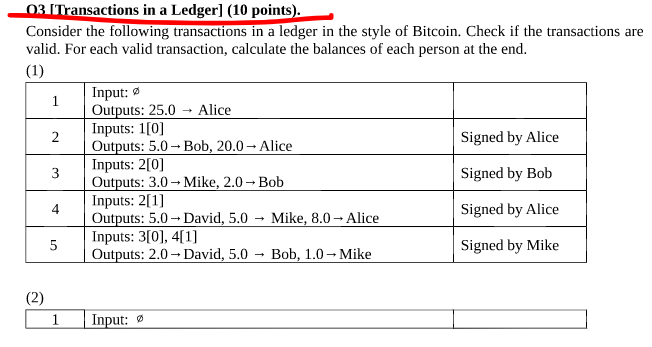
\includegraphics[scale=1]{6.png}\\
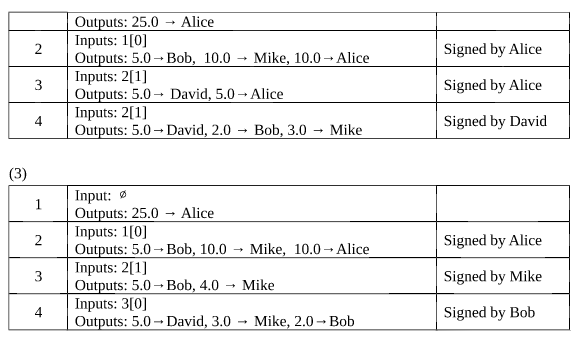
\includegraphics[scale=1]{7.png}\\
1)\\\\
1. Ok
2. Ok
3. Ok mm
4. Ok 2 lost
5. Ok
\\
Alice: 10
Bob: 7
David: 7
Mike: 1
\\\\
2)
\\\\
1. ok
2. ok
3. ok
4. mmm
\\
Alice: 5
Bob: 7
David: 0
Mike: 3
\\\\
3)
\\\\
1. ok
2. ok
3. ok lost 1
4. ok
\\
Alice: 10
Bob: 2
David: 5
Mike: 8

\section{7}
\section{8}







































\end{document}
